% ============================================================
% Section 6 — Does Query-Level Credit Improve Deep Search? (v3, 2026-09-16)
% 数据: HANDOFF §29 (三臂 seed 1 step_100, 有据性链同会话重评, 同题配对),
%       §26-§28 (step 20/50/80 轨迹), §14 + 本窗口复算 (轨迹级覆盖四对配对),
%       ABLATION_TABLES §2 + supp_evals/{singleshot,a3zero,sftv22}_closed_musique (闭池阶梯)
% v2 (2026-09-03, 广播覆盖项为主结果) 的正文以注释保留在各段之后。
% ============================================================

\section{Does Query-Level Credit Improve Deep Search?}
\label{sec:results}

\subsection{Three arms in the training environment}
\label{sec:results-main}

Figure~\ref{fig:arms} compares the three arms of seed 1 at step 100
on the closed-pool MuSiQue development set (full numbers in
Table~\ref{tab:main-qc}, Appendix~\ref{app:main-table}). Query-level credit reaches
51.43 exact match against 47.62 for outcome-only training ($+3.8$; 236
questions flip to correct against 144, $z=4.72$) and 47.46 for the
trajectory-level coverage term ($z=4.94$). Over the outcome-only arm
the gain grows with depth: $+2.5$ at two hops, $+3.3$ at three, and
$+8.9$ at four ($z=4.08$; 57:21). The arm reaches more of the gold set
(final coverage 83.0\% versus 81.2 and 80.4; full-coverage rate 65.1\%
versus 62.9 and 62.5) with fewer search calls (4.31 versus 4.86 and
4.93 per question), and it answers correctly more often both when its
evidence is complete (43.4\% of questions versus 41.0 and 41.7) and
when it is not (7.9\% versus 6.5 and 5.6).

The contrast arms of the other seeds bound the run-level noise. At step
100, outcome-only training reaches 47.62, 47.50, and 47.62 EM over seeds
1--3 and trajectory-level coverage 47.46, 47.46, and 48.74, so the
query-level arm exceeds both by 3.5--3.9 points against a seed spread of
$\pm 0.5$--$0.7$. Along training the arm leads at every evaluated
checkpoint: 46.92 at step 20 (contrast arms 44.15 and 44.52), 51.68 at
step 50 (48.70 and 46.63), 52.50 at step 80 (47.54 and 49.03), and
51.43 at step 100; it searches 0.4--0.6 fewer times per question
throughout.


\begin{figure*}[t]
\centering
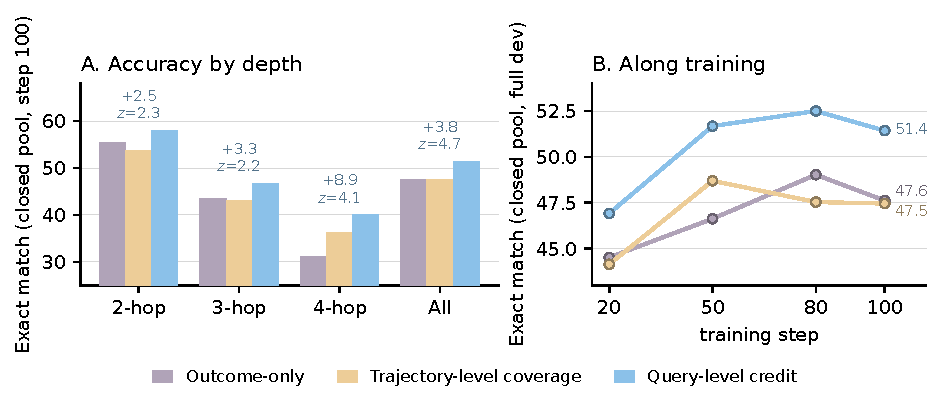
\includegraphics[width=\textwidth]{figs/fig_main_arms.pdf}
\caption{Query-level credit against outcome-only training and the
trajectory-level coverage term on closed-pool MuSiQue dev (seed 1).
(A)~Exact match by depth at step 100; annotations give query-level
credit minus outcome-only and the question-level paired McNemar $z$.
(B)~Full-dev exact match at steps 20, 50, 80, and 100. Per-hop values,
F1, final coverage, and search calls are in Table~\ref{tab:main-qc}
(Appendix~\ref{app:main-table}).}
\label{fig:arms}
\end{figure*}

\subsection{Trajectory-level coverage: four matched pairs}
\label{sec:results-pair}

Table~\ref{tab:main-pair} reports the trajectory-level coverage term
against outcome-only training over four matched pairs of runs (same
SFT initialization, schedule, data order, and rollout samples;
explicit seeds 1--3 and the default seed). Pooled over the four pairs,
4-hop exact match improves by $+3.6$ points (157:99, $z=3.62$); pooled
over the three explicit-seed pairs, by $+2.4$ (116:87, $z=2.04$). The
per-pair 4-hop differences are $+7.2$, $+4.2$, $-2.7$, and $+5.7$
(Fig.~\ref{fig:paired-seeds}). Overall EM moves by $+0.9$ ($z=2.36$;
$+0.6$, $z=1.42$, over the explicit-seed pairs), and search calls per
question are unchanged. The term breaks ties at the level of whole
trajectories and buys a deep-hop gain of this size in the training
environment; \S\ref{sec:mech-broadcast} shows what the broadcast does
at the level of turns, and \S\ref{sec:transfer-traj} what the habit it
teaches costs outside the training environment.
% 原句(v2, 6.1): "Table~\ref{tab:main-pair} reports four matched pairs of runs
% on the closed-pool MuSiQue development set: coverage-shaped RL against
% outcome-only RL ... The effect is depth-structured: pooled over the four
% pairs, $+0.2$ at two hops, $+0.6$ at three, and $+3.6$ at four. ... The
% improvement lands where \S\ref{sec:starvation} locates the all-wrong
% groups."
% 原句(v1, 单对): "Overall exact match improves by $+1.65$ points ($z=2.37$).
% ... $+7.2$ at four hops ($z=3.98$; 41 questions flip to correct against 12
% that flip to wrong). ... $-2.2$ on the easy third, $+1.8$ on the medium,
% $+5.3$ on the hard third ($z=2.72$). ... 4.70 versus 4.98 calls per question
% overall, 6.21 versus 6.56 on 4-hop questions."

\begin{table}[t]
\centering
\small
\resizebox{\columnwidth}{!}{%
\begin{tabular}{lrrrrr}
\toprule
Pair & \multicolumn{2}{c}{Overall EM} & \multicolumn{2}{c}{4-hop EM} & $\Delta$search \\
 & $\Delta$ & $z$ & $\Delta$ & $z$ & \\
\midrule
Seed 1       & $-0.25$ & $-0.31$ & $+4.20$ & $+1.99$ & $+0.10$ \\
Seed 2       & $+0.29$ & $+0.39$ & $-2.72$ & $-1.39$ & $+0.21$ \\
Seed 3       & $+1.82$ & $+2.48$ & $+5.68$ & $+2.81$ & $-0.16$ \\
Default seed & $+1.65$ & $+2.37$ & $+7.16$ & $+3.98$ & $-0.28$ \\
\midrule
Pooled, seeds 1--3 & $+0.62$ & $+1.42$ & $+2.39$ & $+2.04$ & $+0.05$ \\
Pooled, all four   & $+0.88$ & $+2.36$ & $\mathbf{+3.58}$ & $\mathbf{+3.62}$ & $-0.03$ \\
\bottomrule
\end{tabular}}
\caption{Trajectory-level coverage minus outcome-only RL across four
matched pairs (same SFT initialization, schedule, and data order;
explicit seeds 1--3 also share the sampler seed), closed-pool MuSiQue
dev (2{,}417 questions, 405 at four hops), question-level paired McNemar
$z$; $\Delta$search is the difference in search calls per question.}
\label{tab:main-pair}
\end{table}

% ---- Fig 2 占位(fig_paired_seeds.py 待写): 每对一组柱, 4hop ΔEM 与 Δsearch ----
\begin{figure}[t]
\centering
\fbox{\parbox{0.95\columnwidth}{\centering\vspace{2em}
[Figure~2 placeholder: per-pair 4-hop $\Delta$EM and $\Delta$search
for the four matched pairs of Table~\ref{tab:main-pair}, with the
pooled estimate.]\vspace{2em}}}
\caption{Per-pair deep-hop effect of the trajectory-level coverage
term. [Placeholder.]}
\label{fig:paired-seeds}
\end{figure}

\subsection{Run-level variation}
\label{sec:results-seeds}

At the run level, the trajectory-level arms of the three explicit-seed
pairs reach 47.12, 47.83, and 48.49 overall EM ($47.8 \pm 0.7$) with
4-hop EM 34.6, 33.3, and 38.0 ($35.3 \pm 2.4$); the outcome-only arms
reach 47.37, 47.54, and 46.67 ($47.2 \pm 0.5$) with 4-hop EM 30.4, 36.1,
and 32.4 ($32.9 \pm 2.9$). A separate batch of same-seed reruns of the
trajectory-level recipe, which fixes the data order and varies only
training stochasticity, spans $47.5 \pm 1.6$ (Appendix~D). Extended
training of that recipe past the fixed 100-episode endpoint reaches
50.27 EM at episode 120 and degrades beyond it (Appendix~E); the
query-level arm passes that value at step 50.

\subsection{The same-base ladder}
\label{sec:results-ladder}

Table~\ref{tab:ladder} places the result on the ladder of the same
base model in the closed pool. Closed-book answering reaches 4.8 EM; a
single retrieval of the pool's top ten paragraphs 20.8; the search
protocol alone, zero-shot, 23.8; SFT adds 12.2 points over the
zero-shot protocol (411:116, $z=12.85$); outcome-only RL adds 11.2 over
SFT ($z=22.0$); query-level credit adds 3.8 over outcome-only RL
($z=4.72$). At four hops the ladder runs
$1.7 \rightarrow 24.0 \rightarrow 13.3 \rightarrow 18.5 \rightarrow
32.9 \rightarrow 40.0$.\footnote{Ten of the pool's twenty paragraphs
cover half the pool whatever the query, which is why single-shot
retrieval scores above the zero-shot protocol at four hops.}
% 原表(v1/v2): 前三行为开卷(IRCoT 139k)口径 (4.8 / 15.4 / 29.0), SFT 行为
% SFT v3 (34.5); RL 两行 46.55/48.20 (单对) → 47.2/47.8 (种子均值)。
% 原句(v2): "outcome-only RL adds 12.7 points; coverage shaping adds 0.6 on top
% ... 1.7 → 7.9 → 10.1 → 24.9 → 32.9 → 35.3 ... the shaping term accounts for
% 2.4 points of it on the seed means and 3.6 pooled over the four matched pairs."

\begin{table}[t]
\centering
\small
\resizebox{\columnwidth}{!}{%
\begin{tabular}{lccc}
\toprule
Same policy (Qwen3.5-9B), closed pool & EM & 4-hop & F1 \\
\midrule
Closed book                       & 4.8  & 1.7  & 12.6 \\
Single-shot RAG (pool top-10)     & 20.8 & 24.0 & 28.7 \\
Search protocol, zero-shot        & 23.8 & 13.3 & 31.1 \\
SFT                               & 36.0 & 18.5 & 43.1 \\
Outcome-only RL (3 seeds)         & 47.2 & 32.9 & 55.4 \\
Trajectory-level coverage (3 seeds) & 47.8 & 35.3 & 55.9 \\
Query-level credit (seed 1)       & \textbf{51.4} & \textbf{40.0} & \textbf{59.7} \\
\bottomrule
\end{tabular}}
\caption{The same-base ladder on closed-pool MuSiQue dev. Every row is
the same base model under progressively more training; the RL rows of
seeds 1--3 are means, and the query-level row is the seed-1 run of
Table~\ref{tab:main-qc}.}
\label{tab:ladder}
\end{table}

\subsection{Comparison with external systems}
\label{sec:results-external}

Table~\ref{tab:external} places the trained policies against five
search-RL systems reproduced under one retrieval environment. On
wiki18 MuSiQue, query-level credit with continued training against the
open retriever reaches 28.55 EM against 22.09 for ReSearch, the
strongest external system (paired $z=7.80$); on HotpotQA, 48.55 against
45.00 for Search-R1 ($z=3.94$); on the 139k corpus, the
extended-training checkpoint reaches 45.64 against 32.77.

\begin{table*}[t]
\centering
\small
\begin{tabular}{lcccccc}
\toprule
 & \multicolumn{2}{c}{MuSiQue (wiki18)} & HotpotQA (wiki18) & 2Wiki (wiki18) & MuSiQue (139k) \\
System & EM & F1 & EM & EM & EM \\
\midrule
ZeroSearch~\citep{sun2026zerosearch}                     & 9.43  & 16.78 & 30.70 & --- & 11.92 \\
R1-Searcher~\citep{song2025r1searcher}                   & 15.27 & 22.88 & 39.60 & --- & 24.74 \\
StepSearch~\citep{zheng-etal-2025-stepsearch}            & 18.25 & 26.96 & 35.15 & --- & 25.49 \\
Search-R1~\citep{jin2025searchr1}                        & 20.40 & 29.50 & 45.00 & --- & 31.73 \\
ReSearch~\citep{chen2025research}                        & 22.09 & 32.43 & 44.05 & --- & 32.77 \\
\midrule
\rowcolor{shade}
Ours, query-level credit, + 50 episodes against wiki18   & \textbf{28.55} & \textbf{38.81} & \textbf{48.55} & \textbf{44.45} & 44.97 \\
Ours, extended-training checkpoint (Appendix~E)          & 26.52 & 36.90 & 47.15 & 41.75 & \textbf{45.64} \\
\bottomrule
\end{tabular}
\caption{Comparison with search-RL systems under one retrieval
environment (e5-base-v2 over wiki18 or over the 139k-paragraph MuSiQue
pool union); alias EM and F1 on full MuSiQue dev, HotpotQA and 2Wiki on
2{,}000-question subsets.}
% 表注待定(用户 2026-09-16: 先以注释保留):
% External systems are run with their released checkpoints and official
% protocols (Qwen2.5-7B); ours is Qwen3.5-9B. ReSearch and StepSearch are
% trained on MuSiQue; Search-R1 and R1-Searcher on HotpotQA. Question-level
% paired McNemar against the strongest external system on each set:
% MuSiQue vs.\ ReSearch $z=7.80$ (shaded row); HotpotQA vs.\ Search-R1 $z=3.94$. 2Wiki: external systems not yet run (6 evals);
% 139k: outcome-only step-100 arm scores 45.72 (non-paired).
\label{tab:external}
\end{table*}
